%----------------------------------------------------------------------------------------------------------
% 	Copyright (c) 2009 R-forge 'distributions' Core Team, 
% 	
%	The following Sweave code is under the GNU Free Documentation License:
%      	Permission is granted to copy, distribute and/or modify this document
%      	under the terms of the GNU Free Documentation License, Version 1.3
%      	or any later version published by the Free Software Foundation;
%      	with no Invariant Sections, no Front-Cover Texts, and no Back-Cover Texts.
%
%      A copy of the license is included in the 'inst' directory of this package 
%      or on the web at http://www.gnu.org/licenses/licenses.html#FDL
%
%	After running Sweave, the following code could be compiled :
%	  - on windows with a Tex distribution such as miktex (http://miktex.org) 
%		and a front end Latex editor such as texniccenter (http://www.toolscenter.org)
%	  - on mac os with a Tex distribution such as TexLive and a front end Latex
%	  	editor such as Texshop (http://www.uoregon.edu/~koch/texshop/)
%	  - on linux with a Tex distribution such as teTex (http://www.tug.org/teTeX/)
%	  	and a front end Latex editor such as emacs (http://www.gnu.org/software/emacs/)
%
%----------------------------------------------------------------------------------------------------------


\chapter{Classic discrete distribution}
%%%%%%%%%%%%%%%%%%%%%%%%%%%%%%%%%%%%%%%%%%%%%%%%%
\section{Discrete uniform distribution}
\subsection{Characterization}
\begin{wrapfigure}{r}{0.5\textwidth}
  \vspace{-20pt}
  \begin{center}
    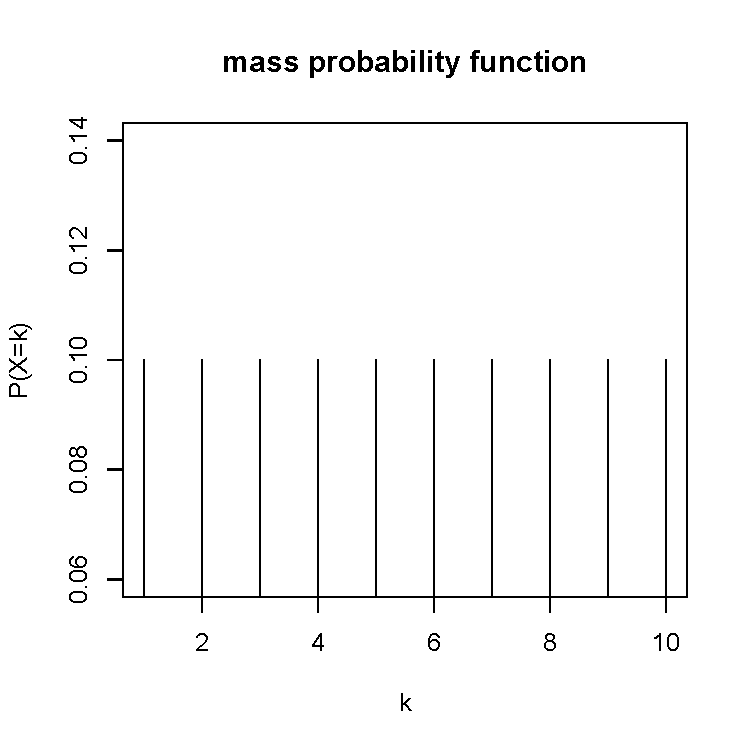
\includegraphics[width=0.48\textwidth]{img/discretunifzoom}
  \end{center}
  \vspace{-20pt}  
  \caption{Mass probability function for discrete uniform distribution}
  \vspace{-20pt}  
\end{wrapfigure}

The discrete uniform distribution can be defined in terms of its elementary distribution
(sometimes called mass probability function):
$$
P(X=k) = \frac{1}{n},
$$
where $k\in S=\{k_1, \dots, k_n\}$ (a finite set of ordered values). Typically, the $k_i$'s are consecutive positive integers.

Equivalenty, we have the following cumulative distribution function:
$$
F(k) = \frac{1}{n} \sum_{i=1}^n \ind_{(k_i\leq k)},
$$
where $\ind$ is the indicator function.

Furthermore, the probability generating function is given by
$$
G(t) \stackrel{\triangle}{=} E(t^X) = \frac{1}{n} \sum_{i=1}^n t^{k_i},
$$
with the special cases where the  $k_i$'s are $\{1,\dots,n\}$, we get
$$
G(t) = z \frac{1-z^n}{1-z},
$$
when  $z\neq 1$.

Finally, the \emph{moment} generating function is expressed as follows
$$
M(t) \stackrel{\triangle}{=} E(t^X) = \frac{1}{n} \sum_{i=1}^n e^{tk_i},
$$
with the special case $e^t \frac{1-e^{tn}}{1-e^t}$ when $S=\{1,\dots,n\}$.


\subsection{Properties}
The expectation is $\overline X_n$, the empirical mean: $ E(X)=\frac{1}{n} \sum_{i=1}^n k_i$.
When $S=\{1,\dots,n\}$, this is just $\frac{n+1}{2}$. The variance is given by $Var(X)=\frac{1}{n} \sum_{i=1}^n (k_i-E(X)^2$ which is $\frac{n^2-1}{12}$ for $S=\{1,\dots,n\}$.

\subsection{Estimation}
Since there is no parameter to estimate, calibration is pretty easy. But we need to 
check that sample values are equiprobable.

\subsection{Random generation}
The algorithm is simply
\begin{itemize}
\item generate $U$ from a uniform distribution,
\item compute the generated index as $I = \lceil n\times U  \rceil$,
\item finally $X$ is $k_I$.
\end{itemize}
where $\lceil . \rceil$ denotes the upper integer part of a number.

\subsection{Applications}
A typical application of the uniform discrete distribution is the statistic procedure called bootstrap or others resampling methods, where the previous algorithm is used.

%%%%%%%%%%%%%%%%%%%%%%%%%%%%%%%%%%%%%%%%%%%%%%%%%
\section{Bernoulli/Binomial distribution}
\subsection{Characterization}
\begin{wrapfigure}{r}{0.5\textwidth}
  \vspace{-20pt}
  \begin{center}
    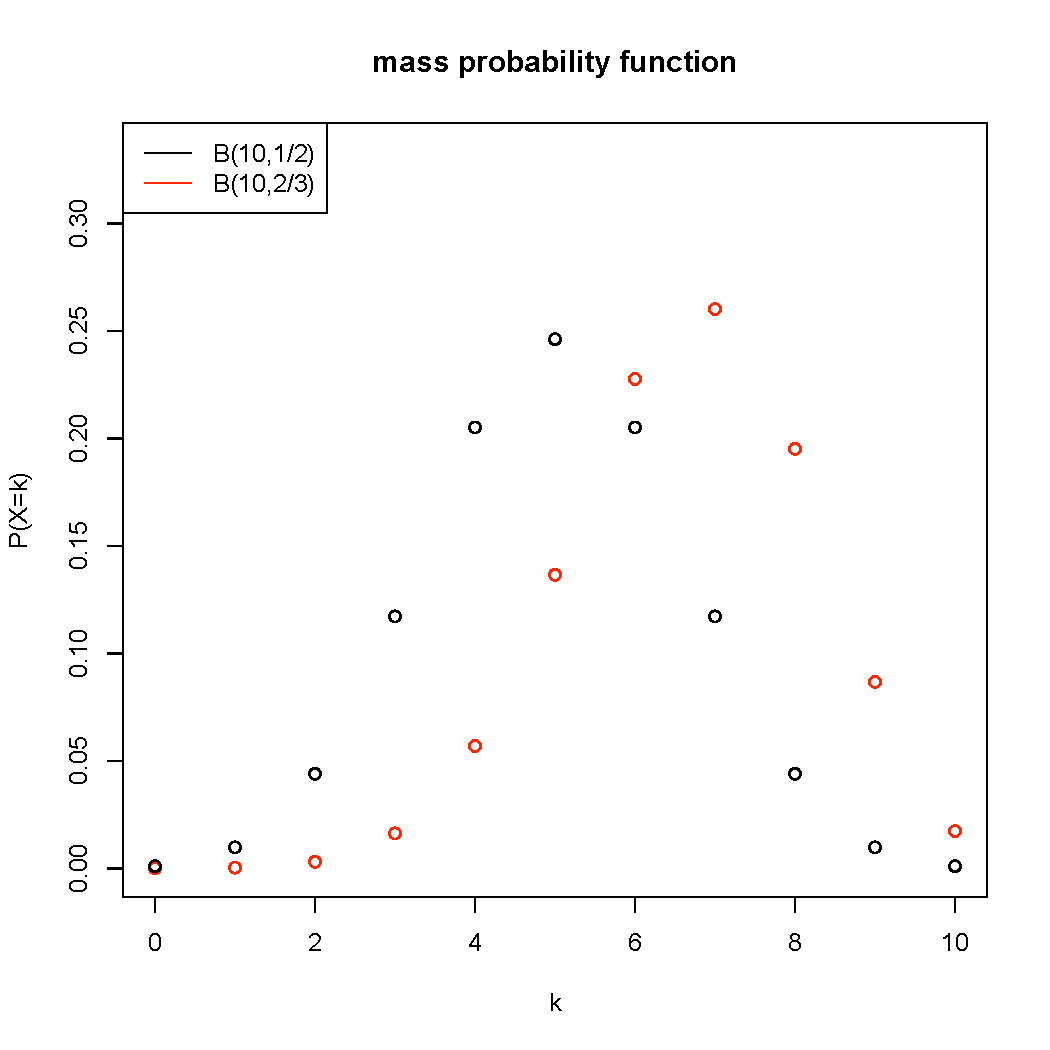
\includegraphics[width=0.48\textwidth]{img/binomzoom}
  \end{center}
  \vspace{-20pt}  
  \caption{Mass probability function for binomial distributions}
  \vspace{-20pt}  
\end{wrapfigure}


Since the Bernoulli distribution is a special case of the binomial distribution, we start by explaining the binomial distribution. The mass probability distribution is 
$$
P(X=k) = C_n^k p^k(1-p)^{n-k},
$$
where $C_n^k$ is the combinatorial number $\frac{n!}{k!(n-k)!}$, $k\in \mathbb N$ and $0<p<1$ the 'success' probability. Let us notice that the cumulative distribution function has no particular expression. In the following, the binomial dsitribuion
is denoted by $\mathcal B(n,p)$. A special case of the binomial dsitribution is the Bernoulli when $n=1$.
This formula explains the name of this distribution since elementary probabilities $P(X=k)$ are terms
of the development of $(p+(1-p))^n$ according the Newton's binom formula.

Another way to define the binomial distribution is to say that's the sum of $n$ identically and independently Bernoulli distribution $\mathcal B(p)$. Demonstration can easily be done with probability generating function.
The probability generating function is
$$
G(t) = (1-p+pz)^n,
$$
while the moment generating function is
$$
M(t) = (1-p+pe^t)^n.
$$

The binomial distribution assumes that the events are binary, mutually exclusive, independent and randomly selected.


\subsection{Properties}
The expectation of the binomial distribution is then $E(X) =np$ and its variance $Var(X)=np(1-p)$. A useful property is that a sum of binomial distributions is still binomial if success probabilities are the same, i.e.
$\mathcal B(n_1, p) + \mathcal B(n_2, p) \stackrel{\mathcal L}{=} \mathcal B(n_1+ n_2, p)$.

We have an asymptotic distribution for the binomial distribution. If $n\rightarrow +\infty$ and $p\rightarrow 0$ such that $np$ tends to a constant, then $\mathcal B(n,p) \rightarrow \mathcal P(np)$.

\subsection{Estimation}
\subsubsection{Bernoulli distribution}
Let $(X_i)_{1\leq i\leq m}$ be an i.i.d. sample of binomial distributions $\mathcal B(n,p)$. If $n=1$ (i.e. Bernoulli distribution, we have 
$$
\hat p_m = \frac{1}{m} \sum_{i=1}^m X_i
$$
is the unbiased and efficient estimator of $p$ with minimum variance. It is also the moment-based estimator.

There exists a confidence interval for the Bernoulli distribution using the Fischer-Snedecor distribution. We have
$$
I_\alpha(p) = \left[ \left(1+\frac{m-T+1}{T} f_{2(m-T+1),2T,\frac{\alpha}{2}}\right)^{-1} , \left(1+\frac{m-T}{T+1} f_{2(m-T),2(T+1),\frac{\alpha}{2}}\right)^{-1} \right],
$$
where $T=\sum_{i=1}^m X_i$ and $f_{\nu_1,\nu_2,\alpha}$ the $1-\alpha$ quantile of the Fischer-Snedecor distribution with $\nu_1$ and $\nu_2$ degrees of freedom.

We can also use the central limit theorem to find an asymptotic confidence interval for $p$
$$
I_\alpha(p) = \left[\hat p_m - \frac{u_\alpha}{\sqrt n} \sqrt{\hat p_m(1-\hat p_m)}, \hat p_m + \frac{u_\alpha}{\sqrt n} \sqrt{\hat p_m(1-\hat p_m)} \right],
$$
where $u_\alpha$ is the $1-\alpha$ quantile of the standard normal distribution.

\subsubsection{Binomial distribution}

When $n$ is not 1, there are two cases: either $n$ is known with certainty or $n$ is unknown.
In the first case, the estimator of $p$ is the same as the Bernoulli distribution. In the latter case, there are no closed form for the maximum likelihood estimator of $n$.

One way to solve this problem is to set $\hat n$ to the maximum number of 'success' at first. Then we compute the log likelihood for wide range of integers around the maximum and finally choose the likeliest value for $n$. 

Method of moments for $n$ and $p$ is easily computable. Equalling the 2 first sample moments, we
have the following solution
$$
\left\{
\begin{array}{l}
\tilde p = 1-\frac{S_m^2}{\bar X_m}\\
\tilde n = \frac{\bar X_m}{\tilde p} 
\end{array}
\right. ,
$$
with the constraint that $\tilde n\in \mbb N$.

Exact confidence intervals cannot be found since estimators do not have analytical form. But we can use the normal approximation for $\hat p$ and $\hat n$.



\subsection{Random generation}
It is easy to simulate Bernoulli distribution with the following heuristic:
\begin{itemize}
\item generate $U$ from a uniform distribution,
\item compute $X$ as 1 if $U\leq p$ and 0 otherwise.
\end{itemize}
The binomial distribution is obtained by summing $n$ i.i.d. Bernoulli random variates.

\subsection{Applications}
The direct application of the binomial distribution is to know the probability of obtaining exactly $n$ heads if a fair coin is flipped $m>n$ times. Hundreds of books deal with this application.

In medecine, the article \cite{nejm} presents an application of the binomial distribution to test for a particular syndrome.

In life actuarial science, the binomial distribution is useful to model the death of an insured or the entry in invalidity/incapability of an insured.

%%%%%%%%%%%%%%%%%%%%%%%%%%%%%%%%%%%%%%%%%%%%%%%%%
\section{Zero-truncated or zero-modified binomial distribution}
\subsection{Characterization}
\begin{wrapfigure}{r}{0.5\textwidth}
 \vspace{-1.5cm}
  \begin{center}
    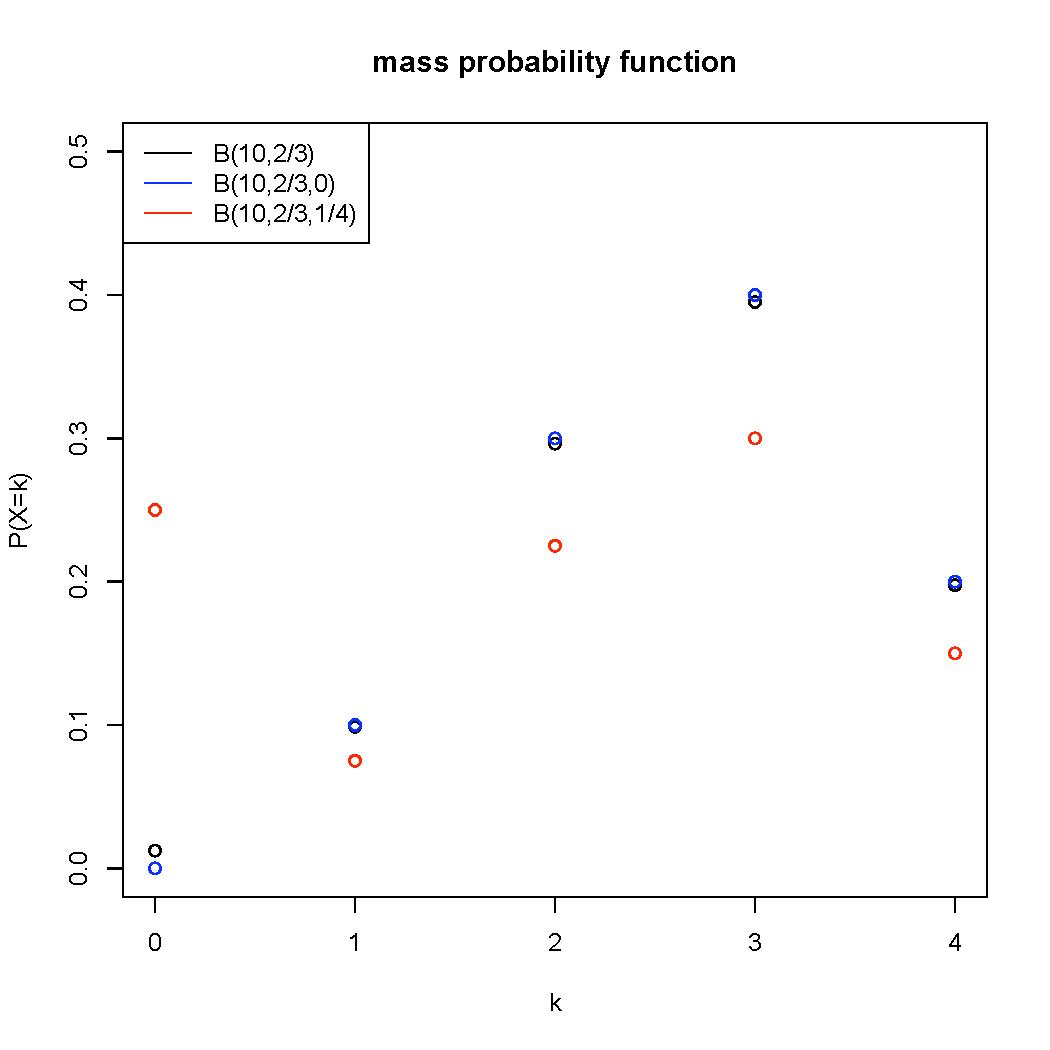
\includegraphics[width=0.48\textwidth]{img/truncbinomzoom}
  \end{center}
  \caption{Mass probability function for zero-modified binomial distributions}
\end{wrapfigure}

The zero-truncated version of the binomial distribution is defined as follows
$$
P(X=k)=\frac{C_n^k p^k (1-p)^{n-k}}{1-(1-p)^n},
$$
where $k\in \{1,\dots,n\}$, $n,p$ usual parameters. The distribution function does not have particular form. But the probability generating function and the moment generating function exist
$$
G(t) = \frac{(1+p(z-1))^n-(1-p)^n}{1-(1-p)^n},
$$
and 
$$
M(t)=\frac{(1+p(e^t-1))^n-(1-p)^n}{1-(1-p)^n}.
$$
In the following distribution, we denote the zero-truncated version by $\mcal B_0(n,p)$.

For the zero-modified binomial distribution, which of course generalizes the zero-truncated version, we have the following elementary probabilities
$$
P(X=k)=\left\{
\begin{array}{ll}
\tilde p &\txtm{if} k=0\\
KC_n^k p^k(1-p)^{n-k}  &\txtm{otherwise}\\
\end{array}
\right.
,
$$
where $K$ is the constant $\frac{1-\tilde p}{1-(1-p)^n}$, $n,p, \tilde p$ are the parameters. In terms of probability/moment generating functions we have:
$$
G(t)=\tilde p + K((1 - p + pz)^n-(1-p)^n) \txtm{and} M(t) = \tilde p + K((1 - p + pe^t)^n-(1-p)^n).
$$
The zero-modified binomial distribution is denoted by $\mcal B(n,p,\tilde p)$.

\subsection{Properties}
The expectation and the variance for the zero-truncated version is $E(X) = \frac{np}{1-(1-p)^n}$ and $Var(X)=\frac{np(1-p-(1-p+np)(1-p)^n)}{(1-(1-p)^n)^2}$. For the zero-modified version, we have $E(X)=Knp$ and $Var(X)=Knp(1-p)$.

\subsection{Estimation}
%\subsubsection{Zero-truncated version}
From \cite{cacoullos}, we know there is no minimum variance unbiased estimator for $p$. NEED HELP for the MLE... NEED \cite{thomasgart}

Moment based estimators are numerically computable whatever we suppose $n$ is known or unknown. 

Confidence intervals can be obtained with bootstrap methods.



\subsection{Random generation}
The basic algorithm for the zero-truncated version $\mcal B_0(n,p)$ is simply
\begin{itemize}
\item \textbf{do}; generate $X$ binomially distributed $\mcal B(n,p)$; \textbf{while} $X=0$
\item return $X$	
\end{itemize}
In output, we have a random variate in $\{1,\dots,n\}$.

The zero-modified version $\mcal B(n,p,\tilde p)$ is a little bit tricky. We need to use the following heuristic:
\begin{itemize}
\item generate $U$ from an uniform distribution
\item if $U< \tilde p$, then $X=0$
\item otherwise 
	\begin{itemize}
	\item \textbf{do}; generate $X$ binomially distributed $\mcal B(n,p)$; \textbf{while} $X=0$
	\end{itemize}
\item return $X$	
\end{itemize}


\subsection{Applications}
Human genetics???

%%%%%%%%%%%%%%%%%%%%%%%%%%%%%%%%%%%%%%%%%%%%%%%%%
\section{Quasi-binomial distribution}
\subsection{Characterization}
The quasi-binomial distribution is a ``small'' pertubation of the binomial distribution. The mass probability function is defined by
$$
P(X=k) = C_n^k p(p+k\phi)^{k-1}(1-p-k\phi)^{n-k},
$$
where $k\in \{0,\dots, n\}$, $n,p$ usual parameters and $\phi\in]-\frac{p}{n},\frac{1-p}{n}[$. Of course, we retrieve the binomial distribution with $\phi$ set to 0.

\subsection{Properties}
NEED REFERENCE
\subsection{Estimation}
NEED REFERENCE
\subsection{Random generation}
NEED REFERENCE
\subsection{Applications}
NEED REFERENCE

%%%%%%%%%%%%%%%%%%%%%%%%%%%%%%%%%%%%%%%%%%%%%%%%%
\section{Poisson distribution}
\subsection{Characterization}
\begin{wrapfigure}{r}{0.5\textwidth}
  \vspace{-20pt}
  \begin{center}
    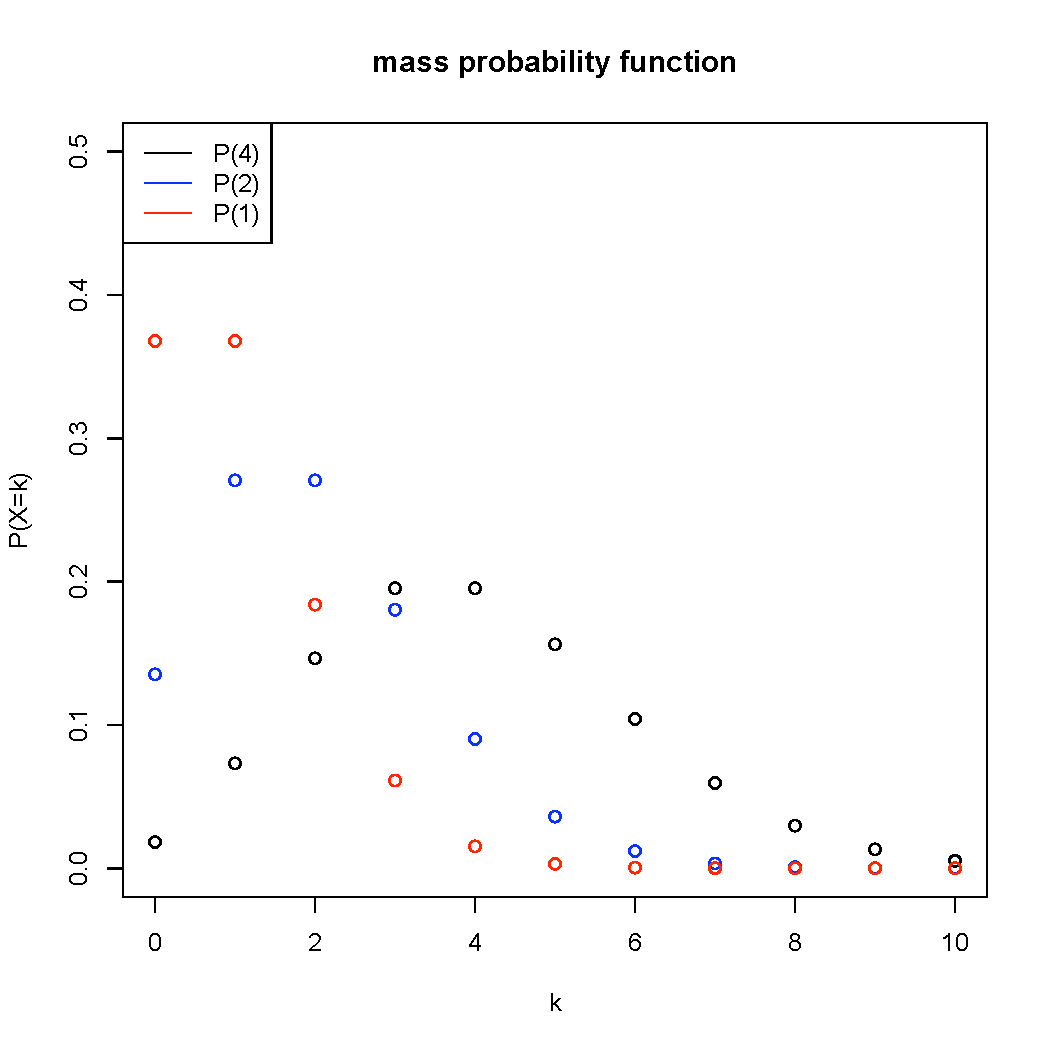
\includegraphics[width=0.48\textwidth]{img/poissonzoom}
  \end{center}
  \vspace{-20pt}
  \caption{Mass probability function for Poisson distributions}
  \vspace{-20pt}
\end{wrapfigure}

The Poisson distribution is characterized by the following elementary probabilities
$$
P(X=k) = \frac{\lambda^k}{k!}e^{-\lambda},
$$
where $\lambda>0$ is the shape parameter and $k\in\mathbb N$.

The cumulative distribution function has no particular form, but the probability generating function is
given by
$$
G(t) = e^{\lambda(t-1)},
$$
and the moment generating function is
$$
M(t) = e^{\lambda(e^t-1)}.
$$

Another way to characterize the Poisson distribution is to present the Poisson process (cf. \cite{saporta}). We consider independent and identically events occuring on a given period of time $t$. We assume that those events can not occur simultaneously and their probability to occur \emph{only} depends on the observation period $t$. Let $c$ be the average number of events per unit of time ($c$ for cadency). We can prove that the number of events $N$ occuring during the period $[0,t[$ is 
$$
P(N=n) = \frac{(ct)^k}{k!}e^{-ct},
$$
since the interoccurence are i.i.d. positive random variables with the property of 'lack of memory'\footnote{i.e. interoccurence are exponentially distributed, cf. the exponential distribution.}.

\subsection{Properties}
The Poisson distribution has the 'interesting' but sometimes annoying property to have the same mean and variance. We have $E(X) = \lambda = Var(X)$.

The sum of two independent Poisson distributions $\mathcal P(\lambda)$ and $\mathcal P(\mu)$ (still) follows a Poisson distribution $\mathcal P(\lambda+\mu)$.

Let $N$ follows a Poisson distribution $\mathcal P(\lambda)$. Knowing the value of $N=n$, let $(X_i)_{1\leq i\leq n}$ be a sequence of i.i.d. Bernoulli variable $\mathcal B(q)$, then $\sum_{i=1}^nX_i$
follows a Poisson distribution $\mathcal P(\lambda q)$.


\subsection{Estimation}
The estimator maximum likelihood estimator of $\lambda$ is $\hat \lambda = \overline X_n$ for a sample $(X_i)_i$. It is also the moment based estimator, an unbiased estimator $\lambda$ and an efficient estimator.

From the central limit theorem, we have asymptotic confidence intervals
$$
I_\alpha(\lambda) = \left[\hat \lambda_n - \frac{u_\alpha}{\sqrt n} \sqrt{\hat \lambda_m} , \hat \lambda_n + \frac{u_\alpha}{\sqrt n} \sqrt{\hat \lambda_m} \right],
$$
where $u_\alpha$ is the $1-\alpha$ quantile of the standard normal distribution.

\subsection{Random generation}
A basic way to generate Poisson random variate is the following:
\begin{itemize}
\item initialize variable $n$ to 0, $l$ to $e^{-\lambda}$ and $P$ to 1,
\item \textbf{do} 
	\begin{itemize}
	\item generate $U$ from a uniform distribution,
	\item $P = P \times U$,
	\item $n=n+1$,
	\end{itemize}
	\textbf{while} $P\geq l$, 
\item return $n-1$.
\end{itemize}
See \cite{knuth02} for details.

 

TOIMPROVE

Ahrens, J. H. and Dieter, U. (1982). Computer generation of Poisson deviates from modified normal distributions. ACM Transactions on Mathematical Software, 8, 163?179.

\subsection{Applications}
TODO


%%%%%%%%%%%%%%%%%%%%%%%%%%%%%%%%%%%%%%%%%%%%%%%%%
\section{Zero-truncated or zero-modified Poisson distribution}
\subsection{Characterization}
\begin{wrapfigure}{r}{0.5\textwidth}
  \vspace{-20pt}
  \begin{center}
    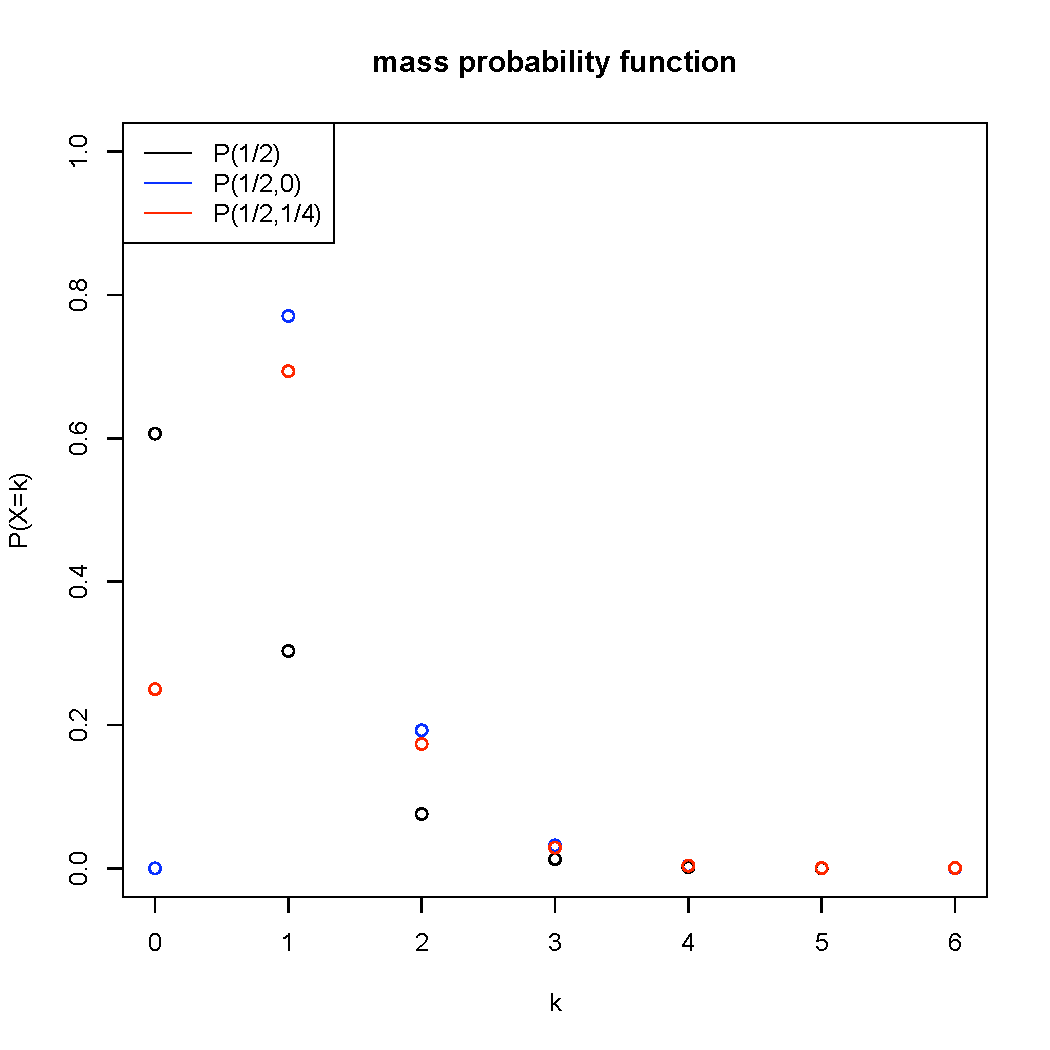
\includegraphics[width=0.48\textwidth]{img/truncpoissonzoom}
  \end{center}
  \vspace{-20pt}
  \caption{Mass probability function for zero-modified Poisson distributions}
  \vspace{-20pt}
\end{wrapfigure}

The zero-truncated version of the Poisson distribution is defined the zero-truncated binomial distribution for the Poisson distribution. The elementary probabilities is defined as
$$
P(X=k)=\frac{\lambda^k}{k!}\frac{1}{(e^\lambda-1)},
$$
where $k\in \mbb N^*$.
We can define probability/moment generating functions for the zero-truncated Poisson distribution $\mcal P_0(\lambda)$:
$$
G(t) = \frac{e^{\lambda t}-1}{e^\lambda-1} \txtm{and} M(t) =\frac{e^{\lambda e^t}-1}{e^\lambda-1}.
$$

The zero-modified version of the Poisson distribution (obviously) generalized the zero-truncated version. We have the following mass probability function
$$
P(X=k)=\left\{
\begin{array}{ll}
p & \txtm{if} k=0\\
K\frac{\lambda^k}{k!} e^{-\lambda} & \txtm{otherwise}
\end{array}
\right.
,
$$
where $K$ is the constant $\frac{1-p}{1-e^{-\lambda}}$. The ``generating functions'' for the zero-modified Poisson distribution $\mcal P(\lambda, p)$ are
$$
G(t)=p+K(e^{\lambda t}-1) \txtm{and} M(t)=p+K(e^{\lambda e^t}-1).
$$


\subsection{Properties}
The expectation of the zero-truncated Poisson distribution is $E(X)=\frac{\lambda}{1-e^{-\lambda}}$ and $K\lambda$ for the zero-modified version. While the variance are respectively $Var(X)=\frac{\lambda}{(1-e^{-\lambda})^2}$ and $K \lambda+(K-K^2)\lambda^2$.

\subsection{Estimation}
\subsubsection{Zero-truncated Poisson distribution}
Let $(X_i)_i$ be i.i.d. sample of truncated Poisson random variables.
Estimators of $\lambda$ for the zero-truncated Poisson distribution are studied in \cite{tategoen}. Here is the list of possible estimators for $\lambda$:
\begin{itemize}
\item $\tilde \lambda = \frac{T}{n}(1-\frac{{}_2S_{n-1}^{t-1}}{{}_2S_{n}^{t}})$ is the minimum variance unbiased estimator,
\item $ \lambda^* = \frac{T}{n}(1-\frac{N_1}{T})$ is the Plackett's estimator,
\item $\hat\lambda$, the solution of equation $\frac{T}{n}=\frac{\lambda}{1-e^{-\lambda}}$, is the maximum likelihood estimator,
\end{itemize}
where $T=\sum_{i=1}^nX_i$, ${}_2S_{n}^{k}$ denotes the Stirling number of the second kind and $N_1$ the number of observations equal to 1. Stirling numbers are costly do compute, see \cite{tategoen} for approximate of theses numbers.

\subsubsection{Zero-modified Poisson distribution}
NEED REFERENCE

\subsection{Random generation}
The basic algorithm for the zero-truncated version $\mcal P_0(\lambda)$ is simply
\begin{itemize}
\item \textbf{do}; generate $X$ Poisson distributed $\mcal P(\lambda)$; \textbf{while} $X=0$
\item return $X$	
\end{itemize}
In output, we have a random variate in $\mbb N^*$.

The zero-modified version $\mcal P(\lambda, p)$ is a little bit tricky. We need to use the following heuristic:
\begin{itemize}
\item generate $U$ from an uniform distribution
\item if $U< p$, then $X=0$
\item otherwise 
	\begin{itemize}
	\item \textbf{do}; generate $X$ Poisson distributed $\mcal P(\lambda)$; \textbf{while} $X=0$
	\end{itemize}
\item return $X$	
\end{itemize}

\subsection{Applications}
NEED REFERENCE

%%%%%%%%%%%%%%%%%%%%%%%%%%%%%%%%%%%%%%%%%%%%%%%%%
\section{Quasi-Poisson distribution}
NEED FOLLOWING REFERENCE

Biom J. 2005 Apr;47(2):219-29.
    Generalized Poisson distribution: the property of mixture of Poisson and comparison with negative binomial distribution.
    Joe H, Zhu R.

    
Ecology. 2007 Nov;88(11):2766-72.
    Quasi-Poisson vs. negative binomial regression: how should we model overdispersed count data?
    Ver Hoef JM, Boveng PL.

 
    
\subsection{Characterization}
TODO
\subsection{Properties}
TODO
\subsection{Estimation}
TODO
\subsection{Random generation}
TODO
\subsection{Applications}

%%%%%%%%%%%%%%%%%%%%%%%%%%%%%%%%%%%%%%%%%%%%%%%%%
\section{Geometric distribution}
\subsection{Characterization}
\begin{wrapfigure}{r}{0.5\textwidth}
  \vspace{-20pt}
  \begin{center}
    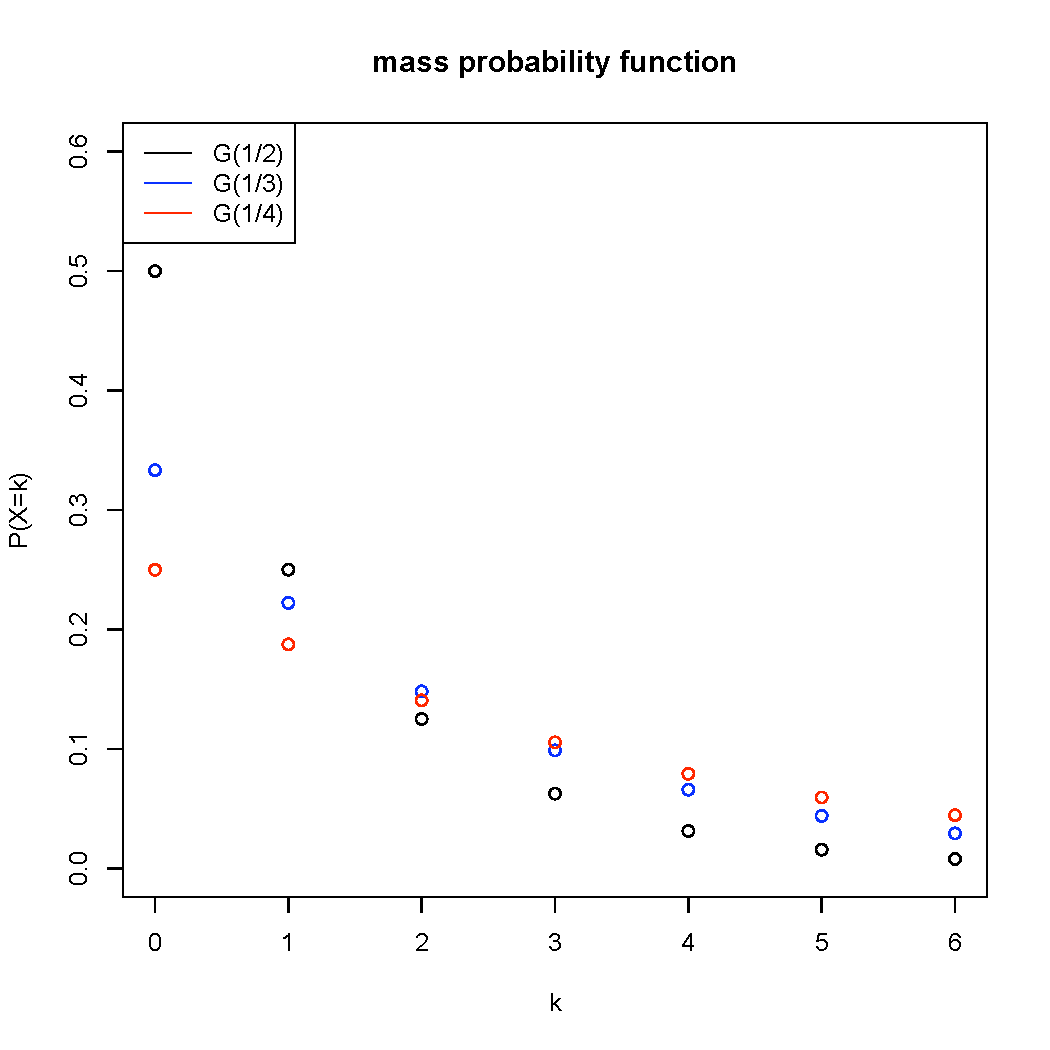
\includegraphics[width=0.48\textwidth]{img/geomzoom}
  \end{center}
  \vspace{-20pt}
  \caption{Mass probability function for Geometric distributions}

\end{wrapfigure}
The geometric distribution represents the first outcome of a particular event (with the probability $q$ to raise) in a serie of i.i.d. events. The mass probability function is 
$$
P(X=k) = q(1-q)^{k},
$$
where $k\in\mathbb N$ and $0<q\leq 1$. In terms of cumulative distribution function, it is the same as
$$
F(k) = 1- (1-q)^{k+1}.
$$
The whole question is wether this outcome could be null or at least one (event). 
If we consider the distribution to be valued in $\mathbb N^*$, please see the truncated geometric distribution.

The probability generating function of the geometric $\mathcal G(q)$ is
$$
G(t) = \frac{q}{1-(1-q)t},
$$ 
and its moment generating function 
$$
M(t) = \frac{q}{1-(1-q)e^t}.
$$

\subsection{Properties}
The expecation of a geometric distribution is simply $E(X)=\frac{1-q}{q}$ and its variance $Var(X)=\frac{1-q}{q^2}$.

The sum of $n$ i.i.d. geometric $\mathcal G(q)$ random variables follows a negative binomial distribution $\mathcal N\mcal B(n,q)$.

The minimum of $n$ independent geometric $\mcal G(q_i)$ random variables follows a geometric distribution $\mcal G(q_.)$ with $q_. = 1-\prod_{i=1}^n (1-q_i)$. 

The geometric distribution is the discrete analogue of the exponential distribution thus it is memoryless. 

\subsection{Estimation}
The maximum likelihood estimator of $q$ is $\hat q = \frac{1}{1+\bar X_n}$, which is also the moment based estimator.

NEED REFERENCE



\subsection{Random generation}
A basic algorithm is to use i.i.d. Bernoulli variables as follows
\begin{itemize}
\item initialize $X$ to 0 and generate $U$ from an uniform distribution,
\item \textbf{while} $U>p$ \textbf{do} ; generate $U$ from an uniform distribution; $X=X+1$; 
\item return $X$.
\end{itemize}
TOIMPROVE WITH 
Devroye, L. (1986) Non-Uniform Random Variate Generation. Springer-Verlag, New York. Page 480. 

\subsection{Applications}
NEED MORE REFERENCE THAN \cite{macutek} 

%%%%%%%%%%%%%%%%%%%%%%%%%%%%%%%%%%%%%%%%%%%%%%%%%
\section{Zero-truncated or zero-modified geometric distribution}
\subsection{Characterization}
\begin{wrapfigure}{r}{0.5\textwidth}
  \vspace{-30pt}
  \begin{center}
    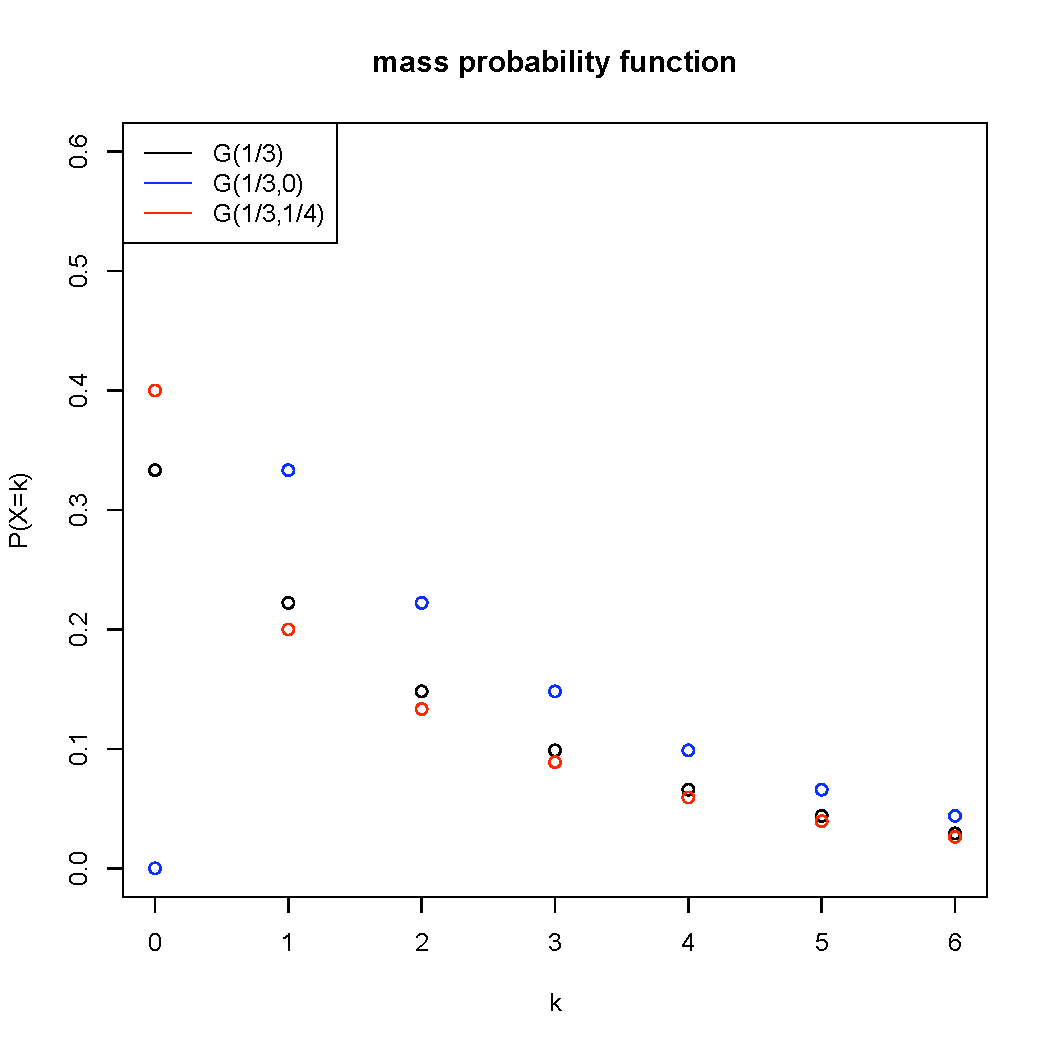
\includegraphics[width=0.48\textwidth]{img/truncgeomzoom}
  \end{center}
  \caption{Mass probability function for zero-modified geometric distributions}
\end{wrapfigure}

The zero-truncated version of the geometric distribution is defined as
$$
P(X=k) = p(1-p)^{k-1},
$$
where $n\in\mathbb N^+$. Obviously, the distribution takes values in $\{1,\dots, n,\dots\}$.
Its distribution function is 
$$
F(k) = 1-(1-p)^k.
$$
Finally the probability/moment generating functions are
$$
G(t) = \frac{pt}{1-(1-p)t}, \txtm{and} M(t) = \frac{pe^t}{1-(1-p)e^t}.
$$
In the following, it is denoted by $\mathcal G_0(p)$.

The zero-modified version of the geometric distribution is characterized as follows
$$
P(X=k) = \left\{
\begin{array}{ll}
p & \txtm{if} k=0\\
Kq(1-q)^k & \txtm{otherwise}\\
\end{array}
\right. ,
$$
where the constant $K$ is $\frac{1-p}{1-q}$ and $k\in\mathbb N$.
Of course special cases of the zero modified version of the geometric $\mathcal G(q,p)$ are the zero-truncated version with $p=0$ and $q=p$ and the classic geometric distribution with $p=q$. The distribution function is expressed as follows
$$
F(x) = p+K(1-(1-p)^k),
$$
where $k\geq 0$. The probability/moment generating functions are 
$$
G(t) = p+K\left(\frac{q}{1-(1-q)t}-q\right) \txtm{and} M(t) =p+K\left(\frac{q}{1-(1-q)e^{t}}-q\right).
 $$

\subsection{Properties}
The expectation of the geometric $\mathcal G_0(p)$ distribution is $E(X)=\frac{1}{p}$ and its variance $Var(X)=\frac{1-p}{p^2}$.

For the zero-modified geometric distribution $\mathcal G(q,p)$, we have $E(X) = K\frac{1-q}{q}$ and $Var(X)=K\frac{1-q}{q^2}$.

\subsection{Estimation}
\subsubsection{Zero-truncated geometric distribution}
According to \cite{cacoullos}, the (unique) minimim variance unbiased estimator of $q$ for the zero-truncated geometric distribution is 
$$
\tilde q = t \frac{\tilde S_n^{t-1}}{\tilde S_n^t},
$$
where $t$ denotes the sum $\sum_{i=1}^n X_i$, $\tilde S_n^t$ is defined by $\frac{1}{n!}\sum_{k=1}^n(-1)^{n-k} C_n^k(k+t-1)_t$\footnote{where $C_n^k$'s are the binomial coefficient and $(n)_m$ is the falling factorial.}. The maximum likelihood estimator of $q$ is given by
$$
\hat q = \frac{1}{\bar X_n},
$$
which is also the moment based estimator. By the uniqueness of the unbiased estimator, $\hat q$ is a biased estimator.

\subsubsection{Zero-modified geometric distribution}
Moment based estimators for the zero-modified geometric distribution $\mcal G(p,q)$ are given by
$\hat q = \frac{\bar X_n}{S_n^2}$ and $\hat p = 1-\frac{(\bar X_n)^2}{S_n^2}$.

NEED REFERENCE

\subsection{Random generation}
For the zero-truncated geometric distribution, a basic algorithm is to use i.i.d. Bernoulli variables as follows
\begin{itemize}
\item initialize $X$ to 1 and generate $U$ from an uniform distribution,
\item \textbf{while} $U>q$ \textbf{do} ; generate $U$ from an uniform distribution; $X=X+1$; 
\item return $X$.
\end{itemize}

While for the zero-modified geometric distribution, it is a little bit tricky
\begin{itemize}
\item generate $U$ from an uniform distribution
\item if $U< p$, then $X=0$
\item otherwise 
	\begin{itemize}
         \item initialize $X$ to 1 and generate $U$ from an uniform distribution
	\item \textbf{while} $U>q$ \textbf{do} ; generate $U$ from an uniform distribution; $X=X+1$;
	\end{itemize}
\item return $X$	
\end{itemize}

\subsection{Applications}
NEED REFERENCE

%%%%%%%%%%%%%%%%%%%%%%%%%%%%%%%%%%%%%%%%%%%%%%%%%
\section{Negative binomial distribution}
\subsection{Characterization}
\subsection{Characterization}
\begin{wrapfigure}{r}{0.5\textwidth}
  \vspace{-30pt}
  \begin{center}
    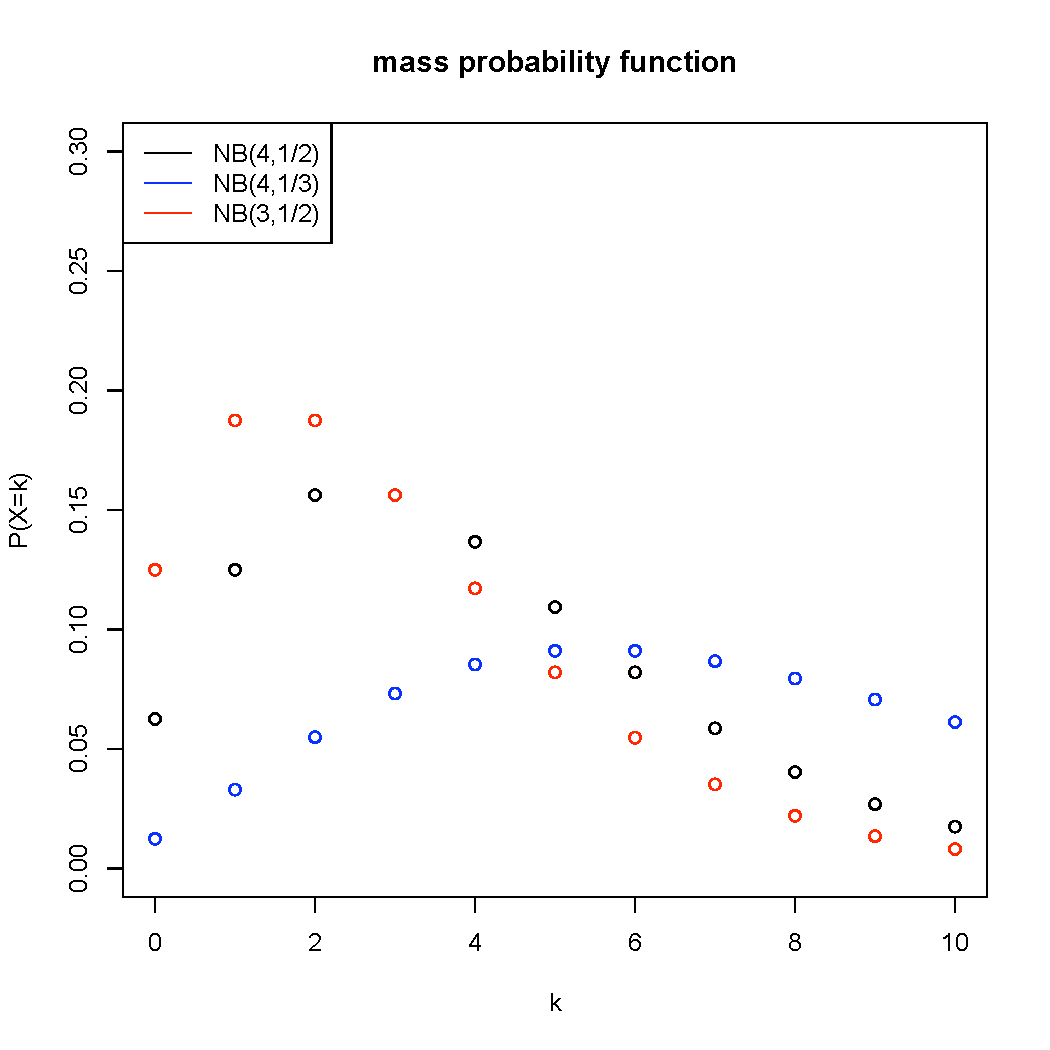
\includegraphics[width=0.48\textwidth]{img/negbinomzoom}
  \end{center}
  \caption{Mass probability function for negative binomial distributions}
\end{wrapfigure}

The negative binomial distribution can be characterized by the following mass probability function
$$
P(X=k) = C_{m+k-1}^{k} p^m(1-p)^{k},
$$
where $k\in\mathbb N$, $C_{m+k-1}^{k}$'s are combinatorial numbers and parameters $m,p$ are constraint by $0<p<1$ and $m\in\mathbb N^*$. However a second parametrization of the negative binomial distribution is
$$
P(X=k)=\frac{\Gamma(r+k)}{\Gamma(r)k!} \left(\frac{1}{1+\beta}\right)^r\left(\frac{\beta}{1+\beta}\right)^k,
$$
where $k\in\mathbb N$ and $r,\beta>0$. We can retrieve the first parametrization $\mathcal N\mathcal B(m,p)$ from the second parametrization $\mathcal N\mathcal B(r,\beta)$ with
$$
\left\{
\begin{array}{c}
\frac{1}{1+\beta} = p\\
r = m\\
\end{array}
\right.
$$

The probability generating functions for these two parametrizations are
$$
G(t)= \left(\frac{p}{1-(1-p)t}\right)^m \txtm{and} G(t)=\left(\frac{1}{1-\beta(t-1)}\right)^r,
$$
and their moment generating functions are 
$$
M(t)= \left(\frac{p}{1-(1-p)e^{t}}\right)^m \txtm{and} M(t) = \left(\frac{1}{1-\beta(e^t-1)}\right)^r.
$$

One may wonder why there are two parametrization for one distribution. Actually, the first parametrization $\mathcal N\mathcal B(m,p)$ has a meaningful construction: it is the sum of $m$ i.i.d. geometric $\mathcal G(p)$ random variables. So it is also a way to characterize a negative binomial distribution.
The name comes from the fact that the mass probability function can be rewritten as
$$
P(X=k) = C_{m+k-1}^{k} \left(\frac{1-p}{p}\right)^{k}\left(\frac{1}{p}\right)^{-m-k},
$$
which yields to
$$
P(X=k) = C_{m+k-1}^{k} P^{k}Q^{-m-k}.
$$
This is the general term of the development of $(P-Q)^{-m}$.
 

\subsection{Properties}
The expectation of negative binomial $\mathcal N\mathcal B(m,p)$ (or $\mathcal N\mathcal B(m,p)$) is $E(X) =  \frac{m(1-p)}{p}$ or ($r \beta$), while its variance is $Var(X)=\frac{m(1-p)}{p^2}$ or ($r\beta(1+\beta)$).

Let $N$ be Poisson distributed $\mathcal P(\lambda\Theta)$ knowing that $\Theta=\theta$ where $\Theta$ is gamma distributed $\mathcal G(a,a)$. Then we have $N$ is negative binomial distributed $\mathcal B\mathcal N(a,\frac{\lambda}{a})$. 



\subsection{Estimation}
Moment based estimators are given by $\hat \beta = \frac{S_n^2}{\bar X_n}-1$ and $\hat r = \frac{\bar X_n}{\hat \beta}$. 

NEED REFERENCE

\subsection{Random generation}
The algorithm to simulate a negative binomial distribution $\mcal N\mcal B(m,p)$ is simply to generate $m$ random variables geometrically distributed and to sum them.

NEED REFERENCE

\subsection{Applications}
From \cite{simon}, here are some applications of the negative binomial distribution
\begin{itemize}
\item number of bacterial colonies per microscopic field,
\item quality control problem,
\item claim frequency in non life insurance.
\end{itemize}

%%%%%%%%%%%%%%%%%%%%%%%%%%%%%%%%%%%%%%%%%%%%%%%%%
\section{Zero-truncated or zero-modified negative binomial distribution}
\subsection{Characterization}
The zero-truncated negative binomial distribution is characterized by
$$
P(X=k) = \frac{\Gamma(r+k)}{\Gamma(r)k!((r+\beta)^r-1)} (\frac{\beta}{1+\beta})^k,
$$
where $k\in \mbb N^*$, $r,\beta$ usual parameters. In terms of probability generating function,
we have
$$
G(t) =  \frac{(1-\beta(t-1))^r-(1+\beta)^{-r}}{1-(r+\beta)^r}.
$$ 

The zero-modified version is defined as follows
$$
P(X=k)=\left\{
\begin{array}{ll}
p & \txtm{if} k=0\\
K\frac{\Gamma(r+k)}{\Gamma(r)k!} (\frac{1}{1+\beta})^r(\frac{\beta}{1+\beta})^k & \txtm{otherwise}\\
\end{array}
\right. ,
$$
where $K$ is defined as $\frac{1-p}{1- (\frac{1}{1+\beta})^r}$, $r,\beta$ usual parameters and $p$ the new parameter. The probability generating function is given by
$$
G(t) = \left((\frac{1}{1-\beta(t-1)})^r-(\frac{1}{1+\beta})^r\right),
$$
and 
$$
M(t) = \left((\frac{1}{1-\beta(e^t-1)})^r-(\frac{1}{1+\beta})^r\right)
$$
for the moment generating function.

\subsection{Properties}
Expectations for these two distribution are $E(X) = \frac{ r \beta}{1-(r+\beta)^r}$ and $Kr \beta$ respectively for the zero-truncated and the zero-modified versions. Variances are $Var(X)=\frac{ r\beta(1+\beta -(1+\beta+r\beta)(1+\beta)^{-r} )}{(1-(r+\beta)^r)^2}$ and $ Kr\beta(1+\beta)+(K-K^2)E^2[X]$.

\subsection{Estimation}
According to \cite{cacoullos}, the (unique) minimim variance unbiased estimator of $p$ for the zero-truncated geometric distribution is 
$$
\tilde p = t \frac{\tilde S_{r,n}^{t-1}}{\tilde S_n^t},
$$
where $t$ denotes the sum $\sum_{i=1}^n X_i$, $\tilde S_n^t$ is defined by $\frac{1}{n!}\sum_{k=1}^n(-1)^{n-k} C_n^k(k+t-1)_t$\footnote{where $C_n^k$'s are the binomial coefficient and $(n)_m$ is the increasing factorial.}. The maximum likelihood estimator of $q$ is given by
$$
\hat q = \frac{1}{\bar X_n},
$$
which is also the moment based estimator. By the uniqueness of the unbiased estimator, $\hat q$ is a biased estimator.

\subsection{Random generation}
\subsection{Applications}

%%%%%%%%%%%%%%%%%%%%%%%%%%%%%%%%%%%%%%%%%%%%%%%%%
\section{Pascal distribution}
\subsection{Characterization}
The negative binomial distribution can be constructed by summing $m$ geometric distributed variables $\mathcal G(p)$. The Pascal distribution is got from summing $n$ geometrically distributed $\mathcal G_0(p)$ variables. Thus possible values of the Pascal distribution are in $\{n, n+1,\dots\}$. The mass probability function is defined as
$$
P(X=k) = C_{k-1}^{n-1} p^n(1-p)^{k-n} ,
$$
where $k\in \{n, n+1, \dots \}$, $n\in \mathbb N^*$ and $0<p<1$. The probability/moment generating functions are 
$$
G(t) = \left(\frac{pt}{1-(1-p)t}\right)^n \txtm{and} M(t) =\left(\frac{pe^{t}}{1-(1-p)e^{t}}\right)^n.
 $$

\subsection{Properties}
For the Pascal distribution $\mathcal Pa(n,p)$, we have
$E(X) = \frac{n}{p}$ and $Var(X)=\frac{n(1-p)}{p^2}$. The link between Pascal distribution $\mathcal Pa(n,p)$ and the negative binomial distribution $\mathcal B\mathcal N(n,p)$ is to substract the constant $n$, i.e. if $X\sim \mathcal Pa(n,p)$ then $X-n\sim \mathcal B\mathcal N(n,p)$.
\subsection{Estimation}
\subsection{Random generation}
\subsection{Applications}

%%%%%%%%%%%%%%%%%%%%%%%%%%%%%%%%%%%%%%%%%%%%%%%%%
\section{Hypergeometric distribution}
\subsection{Characterization}
The hypergeometric distribution is characterized by the following elementary probabilities
$$
P(X=k) =\frac{C_m^kC_{N-m}^{n-k}}{C_N^n},
$$
where $N\in\mathbb N^+$, $(m,n)\in\{1,\dots, N\}^2$ and $k\in \{0,\dots,\min(m,n)\}$. 

It can also be defined though its probability generating function or moment generating function:
$$
G(t) = \frac{C_{N-m}^n\,_2F_1 (-n,-m;N-m-n+1; t) }{C_N^n} \txtm{and} M(t) =\frac{C_{N-m}^n \,_2F_1 (-n,-m;N-m-n+1;e^t)}{C_N^n},
$$
where $\,_2F_1$ is the hypergeometric function of second kind.

\subsection{Properties}
The expectation of an hypergeometric distribution is $E(X) = \frac{nm}{N}$ and $Var(X)=\frac{nm(N-n)(N-m)}{N^2(N-1)}$.

We have the following asymptotic result: $\mathcal H(N,n,m) \mapsto \mathcal B(n,\frac{m}{N})$ when $N$ and $m$ are large such that $\frac{m}{N} \underset{N\rightarrow +\infty}{\longrightarrow} 0<p<1$.

\subsection{Estimation}
\subsection{Random generation}
\subsection{Applications}
Let $N$ be the number of individuals in a given population. In this population, $m$ has a particular property, hence a proportion of $\frac{m}{N}$. If we draw $n$ individuals among this population, the random variable associated with the number of people having the desired property follows a hypergeometric distribution $\mathcal H(N,n,m)$. The ratio $\frac{n}{N}$ is called the survey rate.
